\documentclass[aspectratio=169]{beamer}

\usetheme{Madrid}
\usecolortheme{default}

\usepackage[T1]{fontenc}
\usepackage[utf8]{inputenc}
\usepackage{lmodern}
\usepackage{tikz}
\usepackage{booktabs}
\usetikzlibrary{arrows.meta, positioning}

\title[AgentViz]{AgentViz: Secure LLM-Assisted Data Analysis}
\subtitle{Overview and design decisions}
\author{Maciej Flodzinski}
\date{\today}

\setbeamertemplate{navigation symbols}{}
\setbeamertemplate{footline}[frame number]

\definecolor{agentblue}{RGB}{37, 99, 235}
\definecolor{agentgreen}{RGB}{22, 163, 74}
\definecolor{agentgray}{RGB}{75, 85, 99}

\newcommand{\code}[1]{\texttt{\small #1}}

\begin{document}

\begin{frame}{High-Level Architecture}
  \centering
  \resizebox{0.96\textwidth}{!}{%
  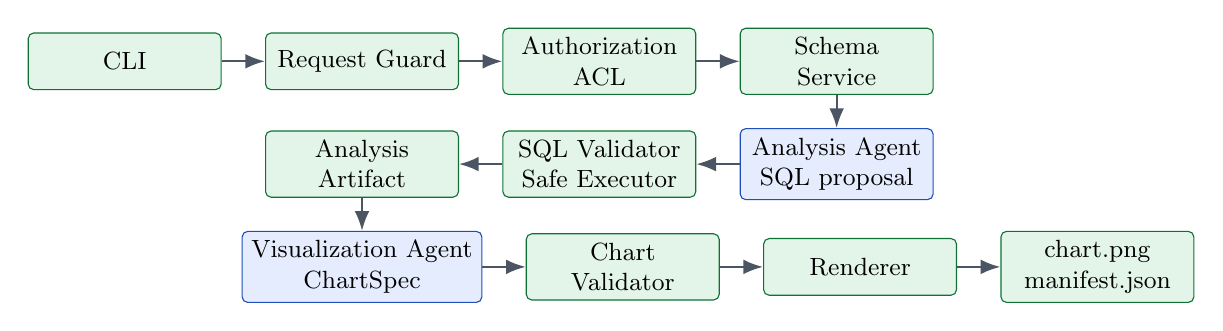
\begin{tikzpicture}[
    node distance=0.42cm and 0.55cm,
    box/.style={
      draw,
      rounded corners=2pt,
      align=center,
      minimum width=2.45cm,
      minimum height=0.72cm,
      font=\small
    },
    det/.style={box, fill=agentgreen!12, draw=agentgreen!70!black},
    llm/.style={box, fill=agentblue!12, draw=agentblue!80!black},
    arrow/.style={-{Latex[length=2.5mm]}, thick, draw=agentgray}
  ]
    \node[det] (cli) {CLI};
    \node[det, right=of cli] (guard) {Request Guard};
    \node[det, right=of guard] (auth) {Authorization\\ACL};
    \node[det, right=of auth] (schema) {Schema\\Service};
    \node[llm, below=of schema] (analysis) {Analysis Agent\\SQL proposal};
    \node[det, left=of analysis] (sql) {SQL Validator\\Safe Executor};
    \node[det, left=of sql] (artifact) {Analysis\\Artifact};
    \node[llm, below=of artifact] (viz) {Visualization Agent\\ChartSpec};
    \node[det, right=of viz] (chartval) {Chart\\Validator};
    \node[det, right=of chartval] (renderer) {Renderer};
    \node[det, right=of renderer] (outputs) {chart.png\\manifest.json};

    \draw[arrow] (cli) -- (guard);
    \draw[arrow] (guard) -- (auth);
    \draw[arrow] (auth) -- (schema);
    \draw[arrow] (schema) -- (analysis);
    \draw[arrow] (analysis) -- (sql);
    \draw[arrow] (sql) -- (artifact);
    \draw[arrow] (artifact) -- (viz);
    \draw[arrow] (viz) -- (chartval);
    \draw[arrow] (chartval) -- (renderer);
    \draw[arrow] (renderer) -- (outputs);
  \end{tikzpicture}
  }

  \vspace{0.35cm}
  \small Green boxes are deterministic. Blue boxes are LLM-backed semantic planners.
\end{frame}

\begin{frame}{LLM Agents}
  \small
  \begin{columns}[T]
    \begin{column}{0.48\textwidth}
      \textbf{Analysis Agent}
      \begin{itemize}
        \item Input: user question plus authorized schema.
        \item Output: structured \code{AnalysisPlan}.
        \item May return \code{query}, \code{clarification}, or \code{unsupported}.
        \item Does not execute SQL.
        \item SQL is validated and executed by deterministic services.
      \end{itemize}
    \end{column}

    \begin{column}{0.48\textwidth}
      \textbf{Visualization Agent}
      \begin{itemize}
        \item Input: row-free visualization context.
        \item Output: declarative \code{ChartSpec}.
        \item Does not generate plotting code.
        \item ChartSpec is validated before rendering.
      \end{itemize}
    \end{column}
  \end{columns}
\end{frame}

\begin{frame}{Design Decisions I}
  \small
  \begin{tabular}{p{0.33\textwidth} p{0.57\textwidth}}
    \toprule
    \textbf{Decision} & \textbf{Reason} \\
    \midrule
    Reject unsafe intent early &
    Request guard rejects obvious destructive or instruction-overriding intent
    before schema access or LLM calls. \\
    \addlinespace
    Authorize before database access &
    ACL policy runs before database connection, schema inspection, SQL
    generation, and execution. \\
    \addlinespace
    Validate SQL after LLM proposal &
    SQL validator allows only read-only SELECT statements over authorized
    schema objects. \\
    \addlinespace
    Validate charts before rendering &
    ChartSpec is validated deterministically before rendering; malformed or
    misleading specs are rejected. \\
    \bottomrule
  \end{tabular}
\end{frame}

\begin{frame}{Design Decisions II}
  \footnotesize
  \begin{tabular}{p{0.34\textwidth} p{0.56\textwidth}}
    \toprule
    \textbf{Decision} & \textbf{Reason} \\
    \midrule
    Structured outputs, not free text &
    Agents must return \code{AnalysisPlan} or \code{ChartSpec}; deterministic
    code can validate and reject malformed model output. \\
    \addlinespace
    Clarification before guessing &
    When key business meaning is missing, the Analysis Agent asks the user and
    the CLI reruns with the answer instead of inventing assumptions. \\
    \addlinespace
    Row-free visualization context &
    The visualization LLM gets column profiles and aggregate statistics, not
    raw rows or potentially malicious cell values. \\
    \addlinespace
    Debuggability without default leakage &
    \code{--save-llm-io} records prompts and structured outputs only when
    explicitly requested, supporting review without always storing prompts. \\
    \bottomrule
  \end{tabular}
\end{frame}

\begin{frame}{Future Improvements}
  \small
  \begin{itemize}
    \item \textbf{Authorization module:} replace the demo username-based ACL with
    real authentication, roles, audit logs, and possibly table/column-level access.
    \item \textbf{Relationship catalog:} persist trusted join hints in config when
    databases do not declare foreign keys, instead of relying on users to repeat
    them in every prompt.
    \item \textbf{Large-schema retrieval:} avoid sending every table to the
    Analysis Agent by first selecting relevant tables/columns deterministically or
    with a smaller schema-search step.
  \end{itemize}
\end{frame}

\end{document}
